\chapter{User Input and Designing}\label{ch:user-input-designer}

\section{Introducion}\label{sec:user-input-introduction}
We started building a GUI by programming every aspect of the interface. We built a \py{MainWindow} class, added some buttons and a plot. A logical next step would be to add a way to change the parameters that build up the scan. We would like to be able to change the \py{start}, \py{stop}, and \py{num_points} values directly from the user interface and not from a config file that gets read-only at the beginning.

We could continue adding elements to the program as we did in the previous chapter, but that is time-consuming. In this chapter, we are going to introduce a program called \textbf{Qt Designer} that is targeted precisely at speeding up the design of user interfaces. We see not only how to make the program better looking, but we are also going to see what happens when we let users input data, what problems may arise, and we show the way to keep improving based on what we achieve by the end of the chapter.

\section{Getting Started with Qt Designer}\label{sec:getting-started-with-qt-designer}
We explained how to install Qt Designer in Section~\ref{sec:install-qt-designer}. Different operating systems and different Python versions have a slightly different way of opening the program.

If you are using \textbf{Anaconda on Windows}, you only have to open the start menu and type \textit{Designer}, press \py{}enter once it finds it. \textbf{Anaconda on Linux} is similar, open a terminal, either from the base environment or the environment used for this book, type \py{designer}, press enter, and a window should open.

If you are using \textbf{plain Python on Windows}, and you installed \py{pyqt5-tools}, you only need to start the \emph{Command Prompt}, activate the environment where you work, type \py{designer.exe}, and press enter. If you are using \textbf{plain Python on Linux}, you installed the Designer as part of the package \py{qttools5-dev-tools}. In this case, the Designer is an actual application that you can find within the installed apps in your distribution.

The Designer welcomes us with a screen like the one below. In between the template/forms options, we can already see two familiar options: Widget and Main Window.

\begin{center}
    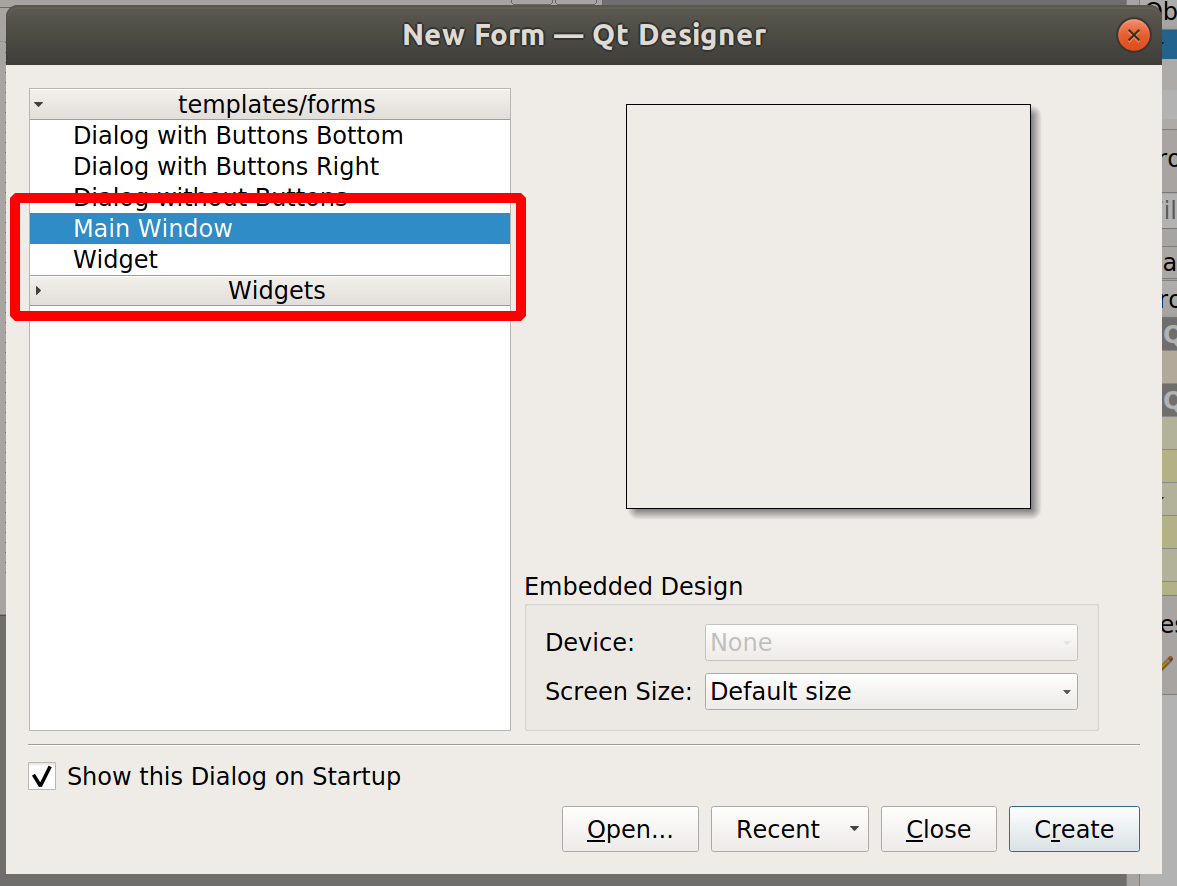
\includegraphics[width=.5\textwidth]{images/Chapter_09/01_Designer_Welcome.png}
\end{center}

We start by recreating the window we developed in the previous chapter. We start by selecting \textbf{Main Window}, and clicking create. The Designer opens the working area with an empty main window. That space is our canvas to start adding elements. In the previous chapter, we created a central widget explicitly. The Designer already did this for us. We can see it on the object inspector at the right sidebar:

\begin{center}
    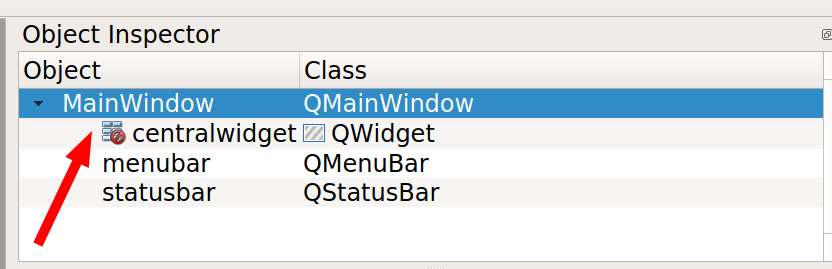
\includegraphics[width=.5\textwidth]{images/Chapter_09/02_central_widget.png}
\end{center}

Note that the Designer named the central widget \py{centralWidget} instead of \py{central_widget}. Naming classes, variables, methods, and functions is completely free in Python, but some conventions make code easier to understand at first sight. One is naming classes with the Camel Case convention, such as \py{MainWindow}, and attributes in lower-case with words separated by underscores. We can change the name of the central widget by clicking on it and changing the \py{objectName} name property:

\begin{center}
    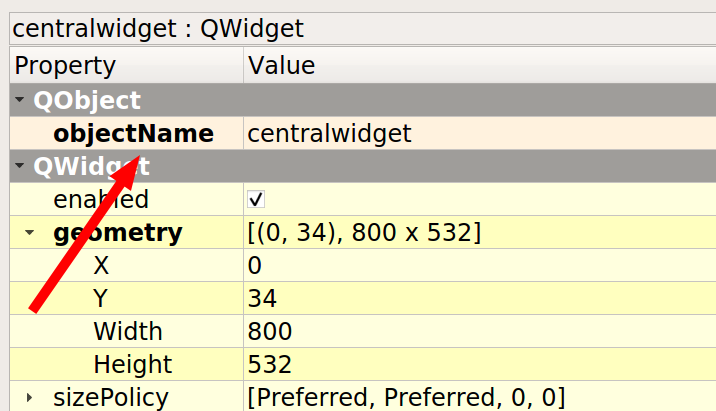
\includegraphics[width=.5\textwidth]{images/Chapter_09/03_central_widget_name.png}
\end{center}

Now we have the central widget with the same name we used in our Python class. We can add the buttons widget by dragging and dropping an empty widget to the window, that can be found in the containers group of elements. After we add the widget, we can also see it appears in the object inspector on the right sidebar. We can change its name to \py{button_widgets}.

\begin{minipage}{0.45\linewidth}
    \centering
    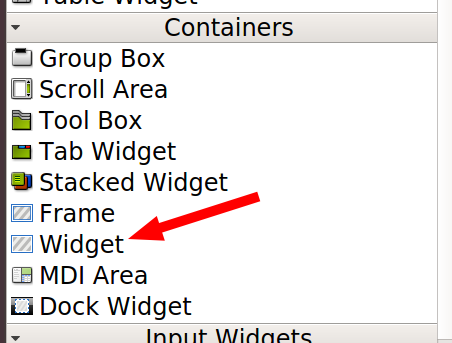
\includegraphics[width=\textwidth]{images/Chapter_09/04_empty_widget.png}
\end{minipage}
\hspace{0.5cm}
\begin{minipage}{0.45\linewidth}
    \centering
    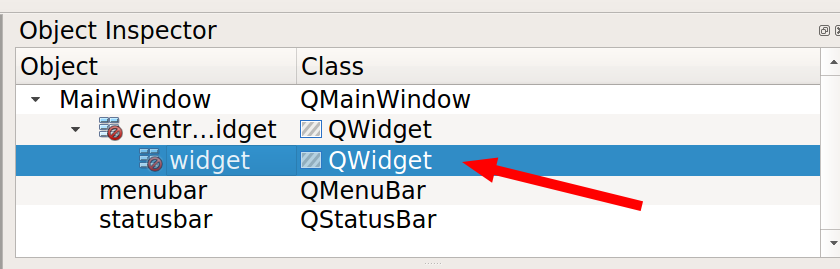
\includegraphics[width=\textwidth]{images/Chapter_09/04_empty_widget_structure.png}
\end{minipage}

To add the start and stop buttons, we can just drag and drop two \py{QPushButton}s to the window. We have to be sure we drop them inside the buttons widget we created earlier. To change the text that appears on the button, we can double click on it and edit the text. We can make one button with the text \emph{Start}, and the other with the text \emph{Stop}. The text on the button is not the name of it. We must change the name of the buttons, and to repeat the same structure of the previous chapter, we are going to call them \py{start_button} and \py{stop_button}. The window and the structure should look like this:

\begin{minipage}{0.45\linewidth}
    \centering
    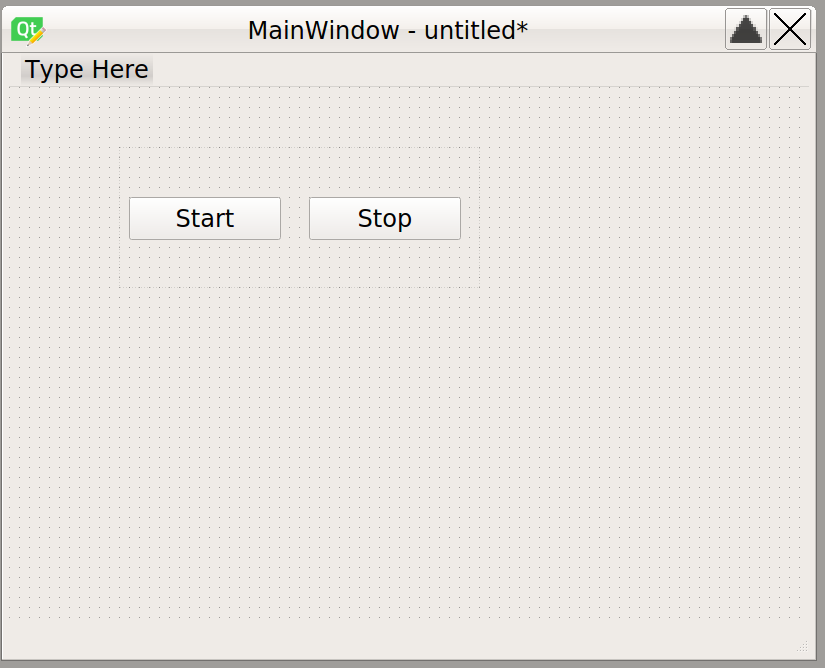
\includegraphics[width=\textwidth]{images/Chapter_09/05_main_window_buttons.png}
\end{minipage}
\hspace{0.5cm}
\begin{minipage}{0.45\linewidth}
    \centering
    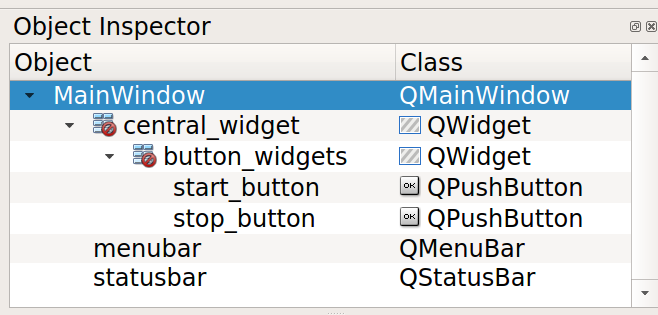
\includegraphics[width=\textwidth]{images/Chapter_09/05_main_window_structure.png}
\end{minipage}

\infoInfo{Screenshots}{Explaining how to use a designing program through screen captures requires much patience from the reader. We try to highlight the checkpoints that allow comparing what the reader does with what we show here. Practice and a critical view is the best that can the reader can do at this stage.}

We have a window with the buttons, but we are missing the layout to make it look as good as we had in the previous chapter. The Designer has a toolbar dedicated exclusively to the layouts; you can find it at the top of the main window space; it looks like this:

\begin{center}
    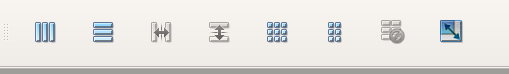
\includegraphics[width=.4\textwidth]{images/Chapter_09/06_layouts.png}
\end{center}

To apply a layout to a widget, we can click first on the widget inside the Object Inspector and then click on the desired layout. We can apply a vertical layout to the \py{central_widget} and a horizontal layout to the \py{button_widgets}. When we apply a layout to widgets, it shows as a different icon on the Object Inspector.

\begin{center}
    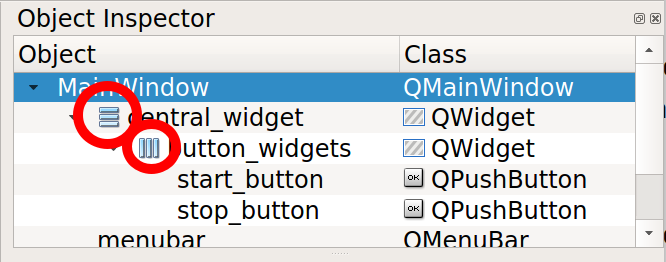
\includegraphics[width=.4\textwidth]{images/Chapter_09/07_widgets_with_layouts.png}
\end{center}

We are ready to save the window. Let's create a new folder called \textbf{GUI} inside the \emph{View} folder, and we can call the file \py{main_window.ui}. Once we save the designer file, we are ready to go back to Python to use this window. We can go back to \textbf{main\_window.py}, and we can start editing the \py{MainWindow} class. Since some of the elements are now defined directly on the designer file, we remove them from the class:

%! Suppress = Ellipsis
\begin{minted}{python}
    import os
    from PyQt5 import uic
    [...]

    class MainWindow(QMainWindow):
        def __init__(self, experiment=None):
            super().__init__()

            base_dir = os.path.dirname(os.path.abspath(__file__))
            ui_file = os.path.join(base_dir, 'GUI', 'main_window.ui')
            uic.loadUi(ui_file, self)

            self.experiment = experiment

            self.plot_widget = pg.PlotWidget()
            self.plot = self.plot_widget.plot([0], [0])
            layout = self.central_widget.layout()
            layout.addWidget(self.plot_widget)
    [...]
\end{minted}

Besides the new imports, the fundamental change to the \py{MainWindow} class is that we load the file using \py{uic.loadUi}. When we try to import files in Python, we always have to be careful with determining the path from which we are importing. We already encountered the syntax of \py{dirname} when we were adding the root folder to the path in Section~\ref{sec:appending-path}. The idea is the same, but we are interested in the folder where the current Python file is located.

The command \py{uic.loadUi} takes two arguments; the first is the file we want to load, and the second is the object to which it is applied. We use the \py{self} to indicate that we want to apply the layout to the entire \py{MainWindow}. If we develop a more modular program, such as defining individual widgets, we could apply the Designer file just to the widget in which we are interested.

The rest of the window stays the same. We only removed the definition of \py{central_widget} and the buttons. Since we have the layout of the central widget specified in the Designer, we need to access it to be able to append the plot widget. It is what this line is doing:

\mint{python}{layout = self.central_widget.layout()}

We can go ahead and run the program, and we see that the window appears as it did before, without changes, even though we are now pulling the elements from the Designer file.

\subsection{Compiling or not Compiling ui files}\label{subsec:compiling-or-not-compiling-ui-files}
Most tutorials online add one step after creating the Designer's file. They normally suggest transforming the \py{.ui} files into a \py{.py} file. There is a program able to do it for us, that can be triggered from the command line:

\begin{minted}{bash}
    pyuic5 main_window.ui -o compiled_window.py
\end{minted}

We can explore both files and see the differences. If we open the \emph{ui} file with a text editor, we find out it is plain text and formatted following a standard called \emph{XML}, or extended markup language. This format is very similar to how websites are built, \emph{HTML} stands for hypertext markup language. Going through the file, we find the place where we defined the buttons, surrounded by some more information, such as the layout, and the text of the button.

If we open the generated Python file, we find the same information but formatted in the same way we have done it in the previous chapter. We can go to the declaration of the start button, and we find a line almost identical to the one we used in the previous chapter

\mint{python}{self.start_button = QtWidgets.QPushButton(self.button_widget)}

The question is whether we \textbf{need} to compile the \emph{ui} files to Python files or not. Qt was developed with C++ programmers in mind, and for a C++ program, it is essential to have each variable defined with a specific type before compiling the code. Qt offers a program, \py{uic} to transform \emph{ui} files to \emph{C++} compatible files. Most Python tutorials built on that experience and kept the recommendation. But for Python, this step is not necessary at all.

There is one caveat, however. If we don't transform the file to a Python file, editors won't be able to know which attributes are available on the windows and widgets. The editor won't have any idea whether there is a \py{start_button} or not defined. It means that to be sure, we should keep opening the designer program and see how we named the buttons and elements. But this is the only drawback that non-compiling has.

In our experience, modifying the designer files and seeing the changes as soon as we restart the program outweighs the problems of not being able to auto-complete. If we are systematic with the naming conventions, we won't face many issues. And if we do encounter issues with attributes not defined, we know that the root of the problem is that we used one name in the Designer and a different one in Python.

\section{Adding User Input}\label{sec:adding-user-input}
\begin{center}
    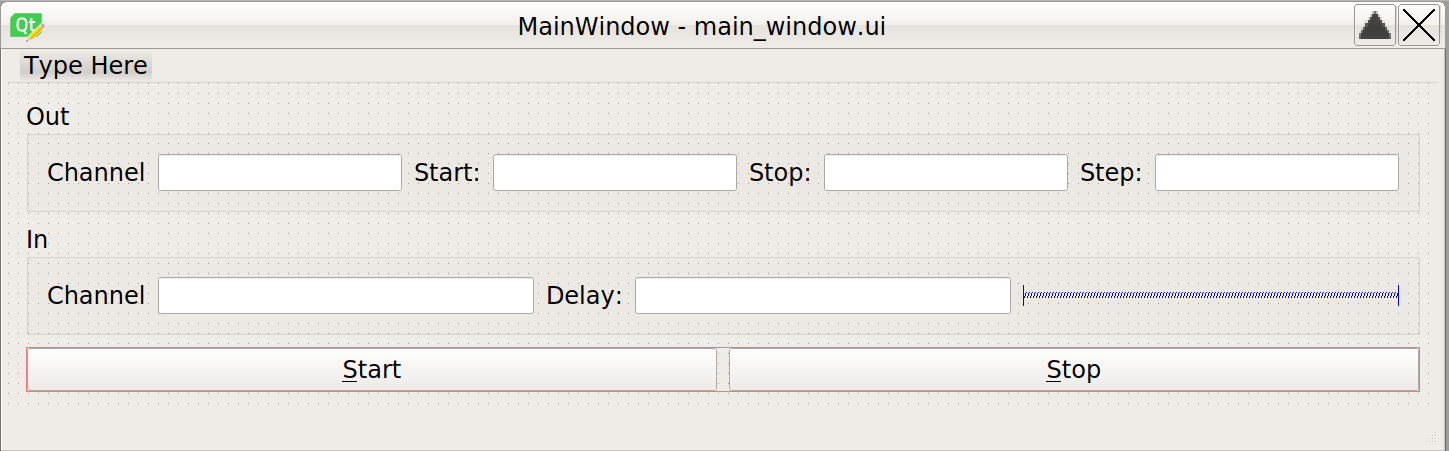
\includegraphics[width=.5\textwidth]{images/Chapter_09/08_final_window_example.png}
\end{center}

It is time to bring our program to the next level by adding the possibility of entering the values of the scan before triggering it. The goal is to have a window that looks like the image above. We structured the window in three rows, one for selecting the range of the scan and the channel, one for the input and delay between points and finally the buttons. Below it, we append the plot, as we have done before.

First, we start by designing the window. We do not cover every single detail as we did in the previous section, because it would become too cumbersome to follow. Therefore we leave to the discretion of the reader whether they want to try it by themselves or get the designer file from the online repository. The easiest way to reproduce the window is by looking at the structure we should obtain after placing all the elements:

\begin{center}
    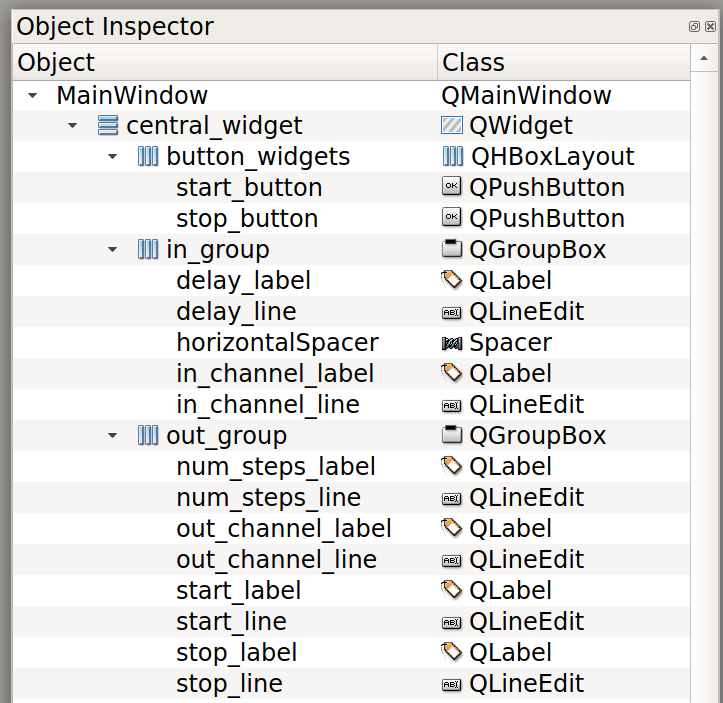
\includegraphics[width=.5\textwidth]{images/Chapter_09/09_final_window_structure.png}
\end{center}

The central widget and the buttons are there, as always, but we added two more widgets now, they are of a particular type called \py{QGroupBox}, meant for grouping elements together. They also have a title that appears at the top left, and become quite handy to understand what we need to edit before starting a scan To handle input from the user, we chose \py{QLineEdit} widgets. These widgets allow the user to input any type of text, precisely as we need.

The rest of the elements are to give consistency to the user experience. Before each line edit, we included a label to show what information is supposed to go in each box. In the bottom group, we also used a \py{Spacer}, to push the elements to the left. If we don't do this, the boxes for editing would take the entire space and wouldn't look cute. It is, however, a purely aesthetic decision.

The most important thing to pay attention to is the names of each input line because they are going to be fundamental for the Python code. What we normally use is a distinctive name followed by the type of element with which we are dealing. That is why have the \py{start_button}, but also the \py{stop_line}, \py{delay_label}, etc. In this way, we can avoid confusion between the starting value of the scan and the button that is supposed to trigger it.

\criticalInfo{Naming Consistency}{Consistency with the names is very important. An incredibly common bug is to change the names and then use the wrong value for the experiment. If we were to swap the in and out channels, the error might go unnoticed until we use two different values. By that point, it is tough to understand if the problem is within the program or within the experiment.}

After improving the window design, we can run again the program and we will see that the window has a different aspect, with inputs, labels and groups. However, they can't do much yet. If we trigger a scan, the plot will update, but it will always be with the values set in the config file. First, let's learn how to populate the different elements with the values we start when we load the config file. We must edit the \py{__init__} of the \py{MainWindow} class to take care of the values:

\begin{minted}{python}
    self.start_line.setText(self.experiment.config['Scan']['start'])
    self.stop_line.setText(self.experiment.config['Scan']['stop'])
    self.num_steps_line.setText(str(self.experiment.config['Scan']['num_steps']))
\end{minted}

The \py{QLineEdit} objects have a method called \py{setText} that allows us to change what is displayed. For the start and stop values, there are no problems, because their values are already strings (remember they include the units), but the number of steps is an integer. PyQt is a very thin wrapper and won't try to convert a number to a string. We need to force it ourselves, adding the \py{str} function.

\questionInfo{Exercise}{We have shown how to add the values of start, stop, and number of steps, but we are still missing the input and output channels, and the delay between points. Add them following the example above.}

We know how to set the values to the lines, we can change them, but the we still use the ones defined in the config file. We already saw in Section~\ref{sec:running-experiment} that thanks to our strategy of having a robust experiment class, we can change the values of the parameters after the experiment was defined. We can do the same within the user interface. Let's improve the \py{start_scan} method of the \py{MainWindow}:

\begin{minted}{python}
    def start_scan(self):
        start = self.start_line.text()
        stop = self.stop_line.text()
        num_steps = int(self.num_steps_line.text())

        self.experiment.config['Scan'].update(
            {'start': start,
             'stop': stop,
             'num_steps': num_steps}
        )
        self.experiment.start_scan()
\end{minted}

In exactly the same way we used \py{setText} to set the text on the QLineEdit objects, we can use \py{text()} to retrieve what is written. For start and stop there are no problems, but for the number of steps we need to have an integer, not a string. Once we got the values, we update the \py{experiment.config}, specifically the group of properties that belong to \py{Scan}. Using \py{update} on a dictionary is a shorter way of doing:

\begin{minted}{python}
    self.experiment.config['Scan']['start'] = start
    self.experiment.config['Scan']['stop'] = stop
    self.experiment.config['Scan']['num_steps'] = num_steps
\end{minted}

It is important to remember that in the experiment, when we trigger the \py{start_scan}, the model takes care of creating the scan range directly from the values stored in the config dictionary. If we supply values without units, the experiment complains.

\questionInfo{Exercise}{Test the limits of the user interface. What happens if you use a number of steps that is not an integer? What happens if you submit a start or stop value in units other than Volts? What happens if you leave one of the options empty?}

\questionInfo{Exercise}{Following the example above, add the same behavior for the delay, channel in and channel out values.}

We are now at a stage where we can control our experiment from the user interface. We can change the parameters for the scan, start, and stop at will. At this stage, we should feel very proud of ourselves. It is also an excellent time to reflect because things change very quickly, new elements appear on the window, but we put minimal effort into making everything work together.

One of the values of separating in Model/View/Controller is that, usually, most of our work should go in the models. And models are the most pure-python modules in our program. Once we overcome the initial shock of working with more complex patterns, such as classes and threads, the rest is very straightforward. We loop through values; we save data. Most likely, it is the kind of things we were already doing when analyzing data.

Once the experiment model is ready, plugging the view on top of it does not require too much effort. How to design the experiment model in such a way that allows us such a degree of independence, is a skill that we can acquire over time, with critical thinking, and patience. For most programs, when developing the \emph{View}, we would face the problem of something missing in the experiment model. Perhaps a threshold value, or a variable that lets us know something is running. We should always refrain from the temptation of complicating the view, and we should always favor putting all that effort into the models.

It's only the long run experience the one that congratulates us on a job well done in the past.

\section{Validating User Input}\label{sec:validating-user-input}
We, as consumers of computer software, are used to a lot of interactions and visual cues when working with a user interface. It makes us expect the same kind of behavior in the programs we develop ourselves. One of the things we can notice in our program is that if we try to trigger a scan while the first one is running, the program prints a message to the terminal, but if we are not paying attention to it, we can miss it and wonder why the scan is not triggering.

One possible solution would be to gray out the \emph{Start} button, to prevent the user from triggering a second scan. The question is, how can we achieve that behavior. If we look in the Designer, every widget that we add has a list of properties that we can change, including shape, color, text. In the case of the buttons, there is an option called \py{enabled}:

\begin{center}
    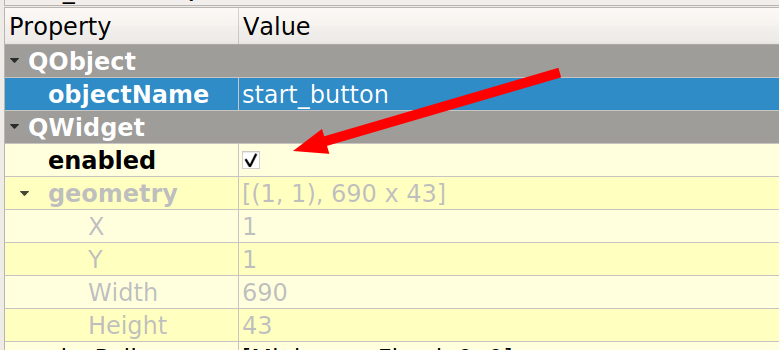
\includegraphics[width=.4\linewidth]{images/Chapter_09/10_enabled_button.png}
\end{center}

If we remove the tick mark from the option, the button gets grayed out, and we won't be able to click it. We must learn how to change the enabled status of our program, not from the Designer. For this, we must read the documentation provided by Qt. If we search online for \py{QPushButton}, usually, the first result would be the one available at \py{doc.qt.io}, the official documentation. We only need to be sure we are looking at the Qt5 documentation and not at the Qt4. The page is long, and if we look for \py{enabled}, we won't find anything. It is not a very auspicious start.

If we scroll to the top of the page, we see that Qt informs us of the parent class of QPushButton: QAbstractButton. Remember that when working with objects, there is always a possibility that methods and attributes are defined in the parent class, not in the class we are using. We can follow the link, but there won't be any information on enabling or not, but if we go one level above, to the \py{QWidget} documentation, we find what we were looking for:

\begin{center}
    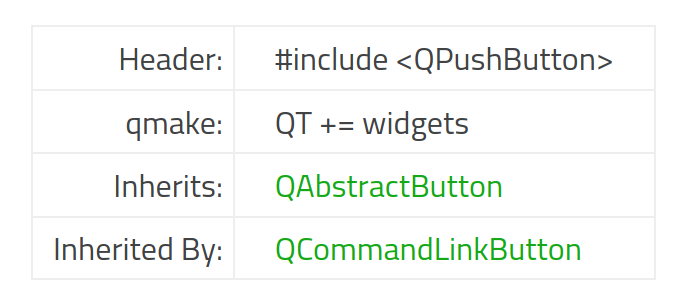
\includegraphics[width=.4\linewidth]{images/Chapter_09/11_Qt_Docs_inheritance.png}
\end{center}

To change the status of the button, we must use the \py{setEnabled()} method that is defined in the base \py{QWidget} class. On the one hand, we can notice that all widgets can be enabled or disabled. In some cases, the change is visible; in others, it won't be. We can also see that the Designer was already letting us know that the documentation was available as part of QWidget instead of QPushButton, just look at how it organizes the properties:

\begin{center}
    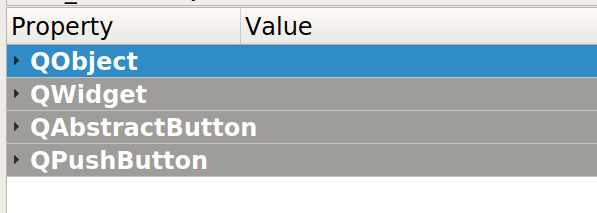
\includegraphics[width=.4\linewidth]{images/Chapter_09/12_Designer_object_inheritance.png}
\end{center}

Next time we want to learn how to do something, we know the best is to start by the Designer and see if the options are available. If we find it, we must pay attention to the base class that defines the behavior, and then we can go looking for the documentation. Navigating the Qt Docs takes a bit of getting used to, but once we understand how the information is organized, it becomes straightforward to follow it.

Back to the task at hand, we must disable the button when the scan starts running. One option would be to disable it right when we trigger the scan:

%! Suppress = Ellipsis
\begin{minted}{python}
    def start_scan(self):
        self.start_button.setEnabled(False)
        [...]
\end{minted}

It seems like a very valid idea until we use it for the first time. Once the scan starts, the button is grayed out, but there is no place where the button can be enabled back. It is a typical pattern with user interfaces. There are different ways to tackle the problem, but the more straightforward one is using the timer we already have in place to update the plot.

Instead of just plotting data, we can use the same timer to update the different elements of the user interface. For example, we would like to let the user start the scan only if there is no scan running, and we want to let them stop the scan only if there is one scan running. Let's start by defining a new method in the main window:

\begin{minted}{python}
    def update_gui(self):
        if self.experiment.is_running:
            self.start_button.setEnabled(False)
            self.stop_button.setEnabled(True)
        else:
            self.start_button.setEnabled(True)
            self.stop_button.setEnabled(False)
\end{minted}

The method \py{update_gui} is easy to follow. If the scan is running, we gray out one button but not the other and vice-versa. We only need to be sure this method runs periodically. Since we already have a timer for updating the plot, we can use it to update the GUI as well:

\begin{minted}{python}
    def __init__(self, experiment=None):
        self.timer.timeout.connect(self.update_gui)
\end{minted}

With this simple approach, we check every few milliseconds whether the scan is running or not, and we set the buttons accordingly. There is also a risk with this approach. If we decide to show information on the Main Window that implies reading a value from the device, we end up polling it several times per second, regardless of whether the value changed or not. If we update values stored in an object, such as the Experiment model, there is nothing to lose, but if we stretch this pattern too far, we may encounter issues, and our program could become inefficient.

We have generated the most basic of the possibilities, disabling a button to prevent the user from triggering a second scan if there is one already running. There are many more possibilities. What happens if the user enters a value outside the range. For example, as a start without volts, or negative, or beyond $3.3\,\textrm{V}$. We can use the \py{update_gui} to monitor the values entered and run them through some checks. If they pass, then we leave them as they are. If they don't, then we change the line to red and disable the start button.

All these are possibilities that we start considering as soon as we start developing user interfaces. However, everything we do has ramifications, such as what we saw when we disabled the start button on our first attempt. Our general approach is not to complicate the user interface beyond what is needed. If we have proper drivers and proper models in place, at least our devices are safe. If we find ourselves or a user of our software, making the same mistakes over and over again, we can then optimize the flow to prevent it from happening again.

\subsection{Saving Data with a Shortcut}\label{subsec:saving-data-with-a-shortcut}
The only missing important feature of our user interface is the ability to save data. We could implement a button for this, but we can also look into another important feature of Qt: \textbf{actions}. We saw that a convenient tool when developing with Qt are signals, such as the ones emitted by a button or a timer. Signals are associated with widgets of some sort. Another range is not associated with widgets, but the user can trigger them at any moment.

In the Designer, we can add a \py{File} menu, by double-clicking the top bar of the main window, where it says \py{Type Here}, and inside the File menu, we can create a \py{Save} option. As soon as we create the Save, the Designer also shows an \emph{Action} defined. We can find the action listed at the bottom of the right sidebar, as we show on the image below. Note that the name assigned by default is \py{actionSave}.

\begin{minipage}{0.45\linewidth}
    \centering
    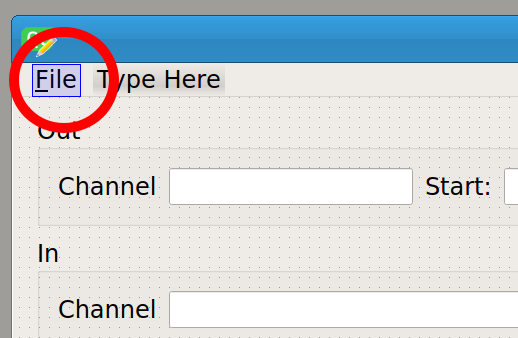
\includegraphics[width=\textwidth]{images/Chapter_09/13_menu_file.png}
\end{minipage}
\hspace{0.5cm}
\begin{minipage}{0.45\linewidth}
    \centering
    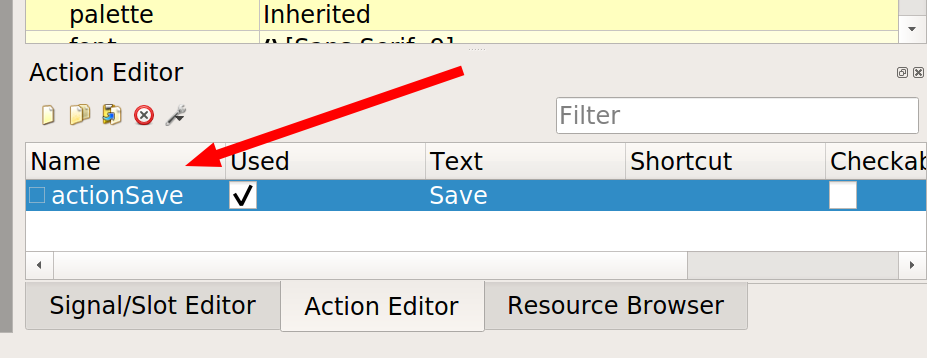
\includegraphics[width=\textwidth]{images/Chapter_09/13_action_save.png}
\end{minipage}

If we pay attention to what appears on that square, we see that there is also the possibility of defining a shortcut. We can go ahead, double-clicking on it opens a small configuration window in which we can add a shortcut, such as Ctrl+S. Just clicking on the shortcut edit line and then pressing a combination of keys register them. After saving, we can rerun the program, and we have a File menu with a Save option, and the shortcut written next to it, so there are no possible confusions.

We need to connect the \py{actionSave} to the method in our experiment for saving data. Because of how we structured the code, this now becomes almost trivial, in the \py{__init__} of the \py{MainWindow} we just add the following:

\mint{python}{self.actionSave.triggered.connect(self.experiment.save_data)}

We can use signals to trigger methods in other objects, not only in the window itself. When the experiment gets more complicated, it can be constructive just to trigger the model to do something than first defining a method on the window to trigger the model then. If we rerun the program, we can save the data either by going to File/Save or by pressing Ctrl+S. Go ahead and check the folder you specified in the config file, and you see the data appearing there.

\tipsInfo{Shortcuts}{Adding shortcuts for actions can be a good idea, but it also has risks. Shortcuts are hard to document, and some shortcuts are so universal that it is better not to re-define them. We could have used Ctrl+S to Start the scan. But then, we need to stop it and choose Ctrl+X, because it is right below. To save, we need to choose another shortcut and choose Ctrl+Q because it is on top of the S. All these shortcuts are generally used for something else, like saving, cutting, and closing a window. We are free to use them as we wish, but over usage leads to a perilous path.}

Of course, we may be tempted to open a pop-up dialog to ask for the folder where to save data. But again, this has a complex set of possibilities. If we open a pop-up every time we want to save data, it becomes annoying, especially if we save data often. If we show it only the first time, then we won't be able to change, later on, wondering why we showed it in the first place. It means we need to establish two behaviors: \emph{save} and \emph{save as}. We won't show how to do it here, but we leave it as an exercise:

\questionInfo{Exercise}{Qt bundles a \py{QFileDialog} widget, which allows the user to select a folder on the computer or create a new one. It can be used like this:

    \py{folder = QFileDialog.getExistingDirectory(self, 'Choose Folder')}.

    Create a new action in the Designer to select the folder, and a new method in the main window to handle the selection of a directory to save the data.}

\section{Conclusions}\label{sec:conclusions}
This chapter is of great joy. It is the conclusion of a great journey, from developing a driver to creating models to abstract the behavior we expect both of the device and of the measurement we want to do, and finally to develop a user interface that works and looks beautiful.

This chapter focused on learning how to use the Qt Designer, a great tool to speed up the development of user interfaces. We covered the essential tools and patterns that one can expect to find in most user interfaces for scientific experiments. Qt, however, is a massive library that allows building almost anything, from the interface you see in some Mercedes cars to coffee vending machines, to programs running right now on your computer or mobile phone.

We have merely scratched the surface of what Qt offers. For scientific applications, however, we don't need to go much deeper. We are generally okay with the simple styling of the objects and a simple menu structure. We can change font-sizes, colors, the roundness of edges. We can make floating menus that open by right-clicking on an image, and many more things. But we always have to draw a line between how much effort and time we are dedicating to making a program look better and how much time we are dedicating to running an experiment.

\section{Where to Next}\label{sec:where-to-next}
If you reached this point, it means that you have kickstarted your career as a Scientific Python Developer, hurrah!. What we have covered in this book is only the beginning. Devices can be much more sophisticated than a simple DAQ, we may need to analyze the data before we display it, or the memory on our computer may not be enough to hold one complete measurement.

Our advice during the workshops is that you should work on what you have learned for at least 6 months—trying to develop solutions for the tools you already have at hand, such as an Oscilloscope, or your own data acquisition card. In this book, we have guided you; we have prevented you from falling in some errors. The reality is that you won't master any technique until you try by yourself, fail by yourself, and solve a problem by yourself.

To accompany you in this process, we have built a forum\footnote{available at: https://forum.pythonforthelab.com}.  You can ask any question related to programming, work in the lab, or Python. If you have any comments, suggestions, compliments, critiques to send us, you can do it directly to me at aquiles@pythonforthelab.com. I always want to read how your path is going, what topics are making you struggle.

If you are interested in a follow-up to this book, covering more advanced topics, please drop me a line. I am always seeking new ideas, topics, challenges, not only to produce content but to learn myself. I do a periodic braindump of what I learn on the website pythonforthelab.com. If anything grabs your attention, you can always leave a comment to let us know.
